%-------------------------------------------------------------------------
\section{Method}
Classic PRT  is a physically-based rendering method to accelerate on-line computations of the (simplified) \textit{Rendering Equation}:
\begin{align}
L(\bm{\omega}_0 ) &= 
\int_{\Omega}   L_{\epsilon}(\bm{\omega}_i ) 
\underbrace{f(\bm{\omega}_i,\bm{\omega}_0) 
V(\bm{\omega}_i) H_N(\omega_i) }_{T(\bm{\omega}_i,\bm{\omega}_0) }
\,  \, d\bm{\omega}_i , 
\label{rendering equation PRT}
\end{align}
where $L_{\epsilon}$ accounts for all incoming radiance over the hemisphere, $f$  describes the surface reflectance properties $f$ (BRDF), $H_N$ is the \textit{Lambert's Law} and $V$ the \textit{Visibility Function} describing geometric information of the scene.\\
It precisely exploits the essence of static/non-deformable objects by uniquely determining the integrand $T(\bm{\omega}_i,\bm{\omega}_0)$ (called the \textbf{\textit{transfer function}} ), which contains the costly-to-compute  \textit{Visibility} term,
\begin{align*}
V :  \mathcal{S}  \times \Omega \rightarrow \{0,1\} \quad,
\end{align*}
for each surface point $\bm{s} \in \mathcal{S} \subset \mathbb{R}^3$ \cite{CohenBook}. 
\\
Both functions $L_{\epsilon} $ and $T$  are projected onto a suitable set of orthonormal basis functions for faster evaluation of the \textit{Rendering Equation} \ref{rendering equation PRT}. 
For $m$ number of coefficients of the basis functions and $l_i$, $t_i$ being the $i$-th coefficient of $L_{\epsilon} $ and $T$ respectively, equation \ref{rendering equation PRT} reduces to \cite{sloan2002precomputed} 
\begin{align}
L(\bm{\omega}_0 ) \approx \sum_{j}^{m} l_j \cdot t_j 
\label{Eq: Reduced Rendering Eq}
\end{align}
We chose a \textit{Spherical Harmonics} (SH) basis to encode the transfer function $T$ and the light environment $L_{\epsilon}$.
\\
\\
 As mentioned above, our aim is to extend the PRT method to malleable and dynamic objects, but avoiding costly pre-computations and storage of every single \textit{transfer function} $T_i$ per shape query $S_i$ (with $i \in [1,2,\dots, d]$ and $d$ : $\#$ deformations ). \\
With this in mind, we suggest a data-based model, a fully Convolutional Neural Network, to infer the \textit{transfer function} $T_i$ for any given shape query $S_i$. \\
This makes the costly ray-casting computations superfluous and solves the abusive memory requirements, only necessitating the storage of the network's parameters. 
%%%%%%%%%%%%%%%%%%%%%%%%%%%%%%%%%%
% -------------- GEOMETRY IMAGE ----------------- 
%%%%%%%%%%%%%%%%%%%%%%%%%%%%%%%%%%
\subsection{Data: Geometry Images}
We propose learning directly \textbf{on} the object's surface in order to leverage its underlying shape structure. \textit{Geometry images} present a planar shape representation on which standard 2D CNNs can be applied \cite{gu2002geometry, sinha2016deep}. 
\\ 
Surfaces with a single boundary (topological disks) are mapped onto a unit square and later discretised (or resampled) into a regular grid of $n \times n$ vertices. \\
In \textit{geometry images} a \textit{Stretch-Minimising} parametrisation is presented for the interior of the planar surface. However, for simplicity, but without loss of generality, we  chose a \textit{Harmonic Map}, based on \cite{HM_book, HarmonicMapping}. \\
\\
It is to note that we apply deformations only on the reconstructed object (right shape of Figure (\ref{Fig: Teaser}) ) in order to make our shape representation, \textit{geometry images}, invariant to deformations. By doing so, we maintain a one-to-one pixel correspondence; hence, filtering out deformation invariant information of the surface; and therefore, facilitating the feature extraction of surface properties that are more related to self-shadowing effects. 
\\
Moreover, this means that the conversion process of a surface into a geometry image has to be performed just once and can be done off-line, saving precious computation time.\\
\\
The surface information we transform into \textit{geometry images} to use as regressor for the CNN are: vertex positions $\mathcal{P}$ and normals $\mathcal{N}$. 
\begin{align*}
	\mathcal{P} = [ P_x, P_y, P_z ]^T , \quad
	\mathcal{N} = [ N_x, N_y, N_z ] ^T 
\end{align*}
with  $P_i, N_i \in \mathbb{R}^{n \times n }$ being the position and normal images, respectively, for each coordinate $i \in \{ x,y,z\}$.
\\
\\
Resulting, our CNN model predicts a corresponding sequence of images $\mathcal{T_{C,R}}$,
\begin{align*}
	f_{CNN} (  \mathcal{P} , \mathcal{N} ) = 
	\begin{cases}
	\mathcal{T_D}  & \text{diffuse} \\
	\mathcal{T_G} & \text{glossy}
	\end{cases},
\end{align*}
which, for \textbf{diffuse materials}, consists of the SH-coefficients of the \textit{transfer function} of the input shape, as introduced above (see equation \ref{Eq: Reduced Rendering Eq}):
\begin{align*}
	\mathcal{T_D} = [ t_1, t_2, \dots, t_m ]^T \in \mathbb{R}^{m \times n \times n} 
\end{align*}
that is, vertex $i$ of image $t_j$ represents the transfer coefficient $j$ of vertex $i$ of the input surface.
\\
For \textbf{glossy materials}, our network predicts the transfered radiance $\mathcal{T_G}$ consisting of three radiance channels, 
\begin{align*}
\mathcal{T_G} = [T_r , T_g ,T_b]^T \in \mathbb{R}^{3 \times m \times n \times n} 
\end{align*}
resulting from the product between the transfer matrix $M_T$ and the lighting coefficients  $ L^{sh}_i$ \cite{sloan2002precomputed}. 
\begin{align*}
T_i= M_T \cdot L^{sh}_i   \in \mathbb{R}^{m \times n \times n}   \quad \text{forx }~  i \in \{r,g,b\} 
\end{align*}
%%%%%%%%%%%%%%%%%%%%%%%%%%%%%%%%%%
% -------------- NETWORK ----------------- 
%%%%%%%%%%%%%%%%%%%%%%%%%%%%%%%%%%
\subsection{Network and Performance }
\subsubsection*{Architecture: \\} 
The topology of our deep convolutional network is based on a \textit{U-Net}  \cite{U-Net}, consisting of an Encoder and Decoder with Skip-Connections. Both Encoder and Decoder consist of sequences of ResNet blocks \cite{ResNet} each comprising a series of 2D-Convolution, Batch Normalisation and ReLU - Activation layers (illustrated in Figure (\ref{Fig: NetworkTopology}) ). For the last layer of the decoder we use a Sigmoid-Activation-Function. Instead of a Pooling-Layer we perform down-sampling by increasing the stride, by a factor of two, within a Convolutional layer \cite{StridingConv}. To avoid information loss,  we make use of Skip-Connections passing information between outputs of encoding layers and corresponding inputs of the decoding layers.

\subsubsection*{Synthesis of Training Data :\\}
We generate the training data applying a sequence of free form deformations onto a given object. Specifically, for our experiments, deformations are generated either by a physically driven simulation or by a blendshape based animation (see Section ?? for examples). Each generated deformation sequence has a total length of 500 frames. 
\\
At each frame $i \in [1,2,\dots,500]$ we store the position $\mathcal{P}_i$  and normal $\mathcal{N}_i$ images of the current deformation , and perform a full self-shadowing integration using ray-casting to compute and store the corresponding ground truth transfer coefficients ($\mathcal{T_D}_i$ or $\mathcal{T_G}_i$). For our experiments we chose a SH-band number of $4$, which corresponds to $16$ coefficients. Moreover, as mentioned above with image resolutions of $256 \times 256$ and $512 \times 512$. 
\\
Our implementation for the generation of the ground truth data $\mathcal{T_{D,G}}$ requires, per frame, a duration of $39.6$s for diffuse and $49.7$s for glossy surfaces.

\subsubsection*{Training: \\} 
The data is split into a training and validation set consisting of 450 and 50 data samples respectively. As cost function, we minimize the pixel-wise absolute error between predicted output and the ground-truth ($L_1$-loss), and the optimizer we use is ADAM \cite{ADAM}. 
\\
Convergence varies from object to object, but in most cases 500 to 1000 epochs are sufficient, whereby a we used a batch size of 5. \\
The network is implemented in Keras with Tensorflow as Backend \cite{Keras} and takes close to 16 hours to compute 800 epochs of training on a single NVIDIA GetForce GTX 2080 GPU.

\subsubsection*{DeepPRT Performance: \\}
In order for \textit{DeepPRT} to function in real-time, fast network inference is required. However, to achieve high accuracies, existing deep convolutional network models, such as ours, rely on very deep architectures with millions of parameters. 
\\
In particular, our network has an approximate amount of $11.8$ million parameters, occupying $45$Mbytes of space, and with an inference time close to $45$ms on a high-end GPU \textit{NVIDIA RTX 2080}. \\
Besides, for a network input size of $4.5$Mbytes there is an additional loading\footnote{Loading six input images, $\mathcal{P}$ and $\mathcal{N}$, into the GPU} cost of approximately $5$ms.  
\\
\\
After prediction, the performance for the rendering process differs significantly between diffuse and glossy surfaces:
\\ 
For \textbf{diffuse} surfaces, the dot product between predicted transfer coefficients $\mathcal{T_D}$ and the three channels of the lighting coefficients is calculated (eq. \ref{Eq: Reduced Rendering Eq}) and the result passed to the buffers for final rendering.  For our sample geometries with $256^2$ number of vertices the computation of the dot product takes $13$ms on the GPU, and a loading time of $0.09$s for the resulting $4.0$Mbytes exiting radiance vectors.
\\ 
On the other hand, for the same sample geometry, to render a \textbf{glossy} surface, the netowrk prediction $\mathcal{T_G}$, of size $12.0$Mbytes, needs to be convolved with a BRDF-kernel before passed to the shaders \cite{sloan2002precomputed}.  We perform this steps in the CPU based on \cite{ BRDF_kernel}, with a resulting total duration of $1.29$s. 
\\
We note that our implementation is far from being optimal.  Both, the rendering and the prediction process can be accelerated significantly. It has been extensively shown that most neural network models are highly compressible and can be significantly accelerated, eventually making them deployable to devices with low memory resources and applicable in real-time \cite{Deep_Compression, Survey_NN_Compression}.
Nevertheless, exploring network optimisation methods reaches beyond the scope of this work. Hence, for our experiments we used the uncompressed CNN introduced above. In section [??] we show that even neglecting network optimisations our DeepPRT-approach already achieves immense memory savings. 
%%%%
\begin{figure*}[t]
  \centering
    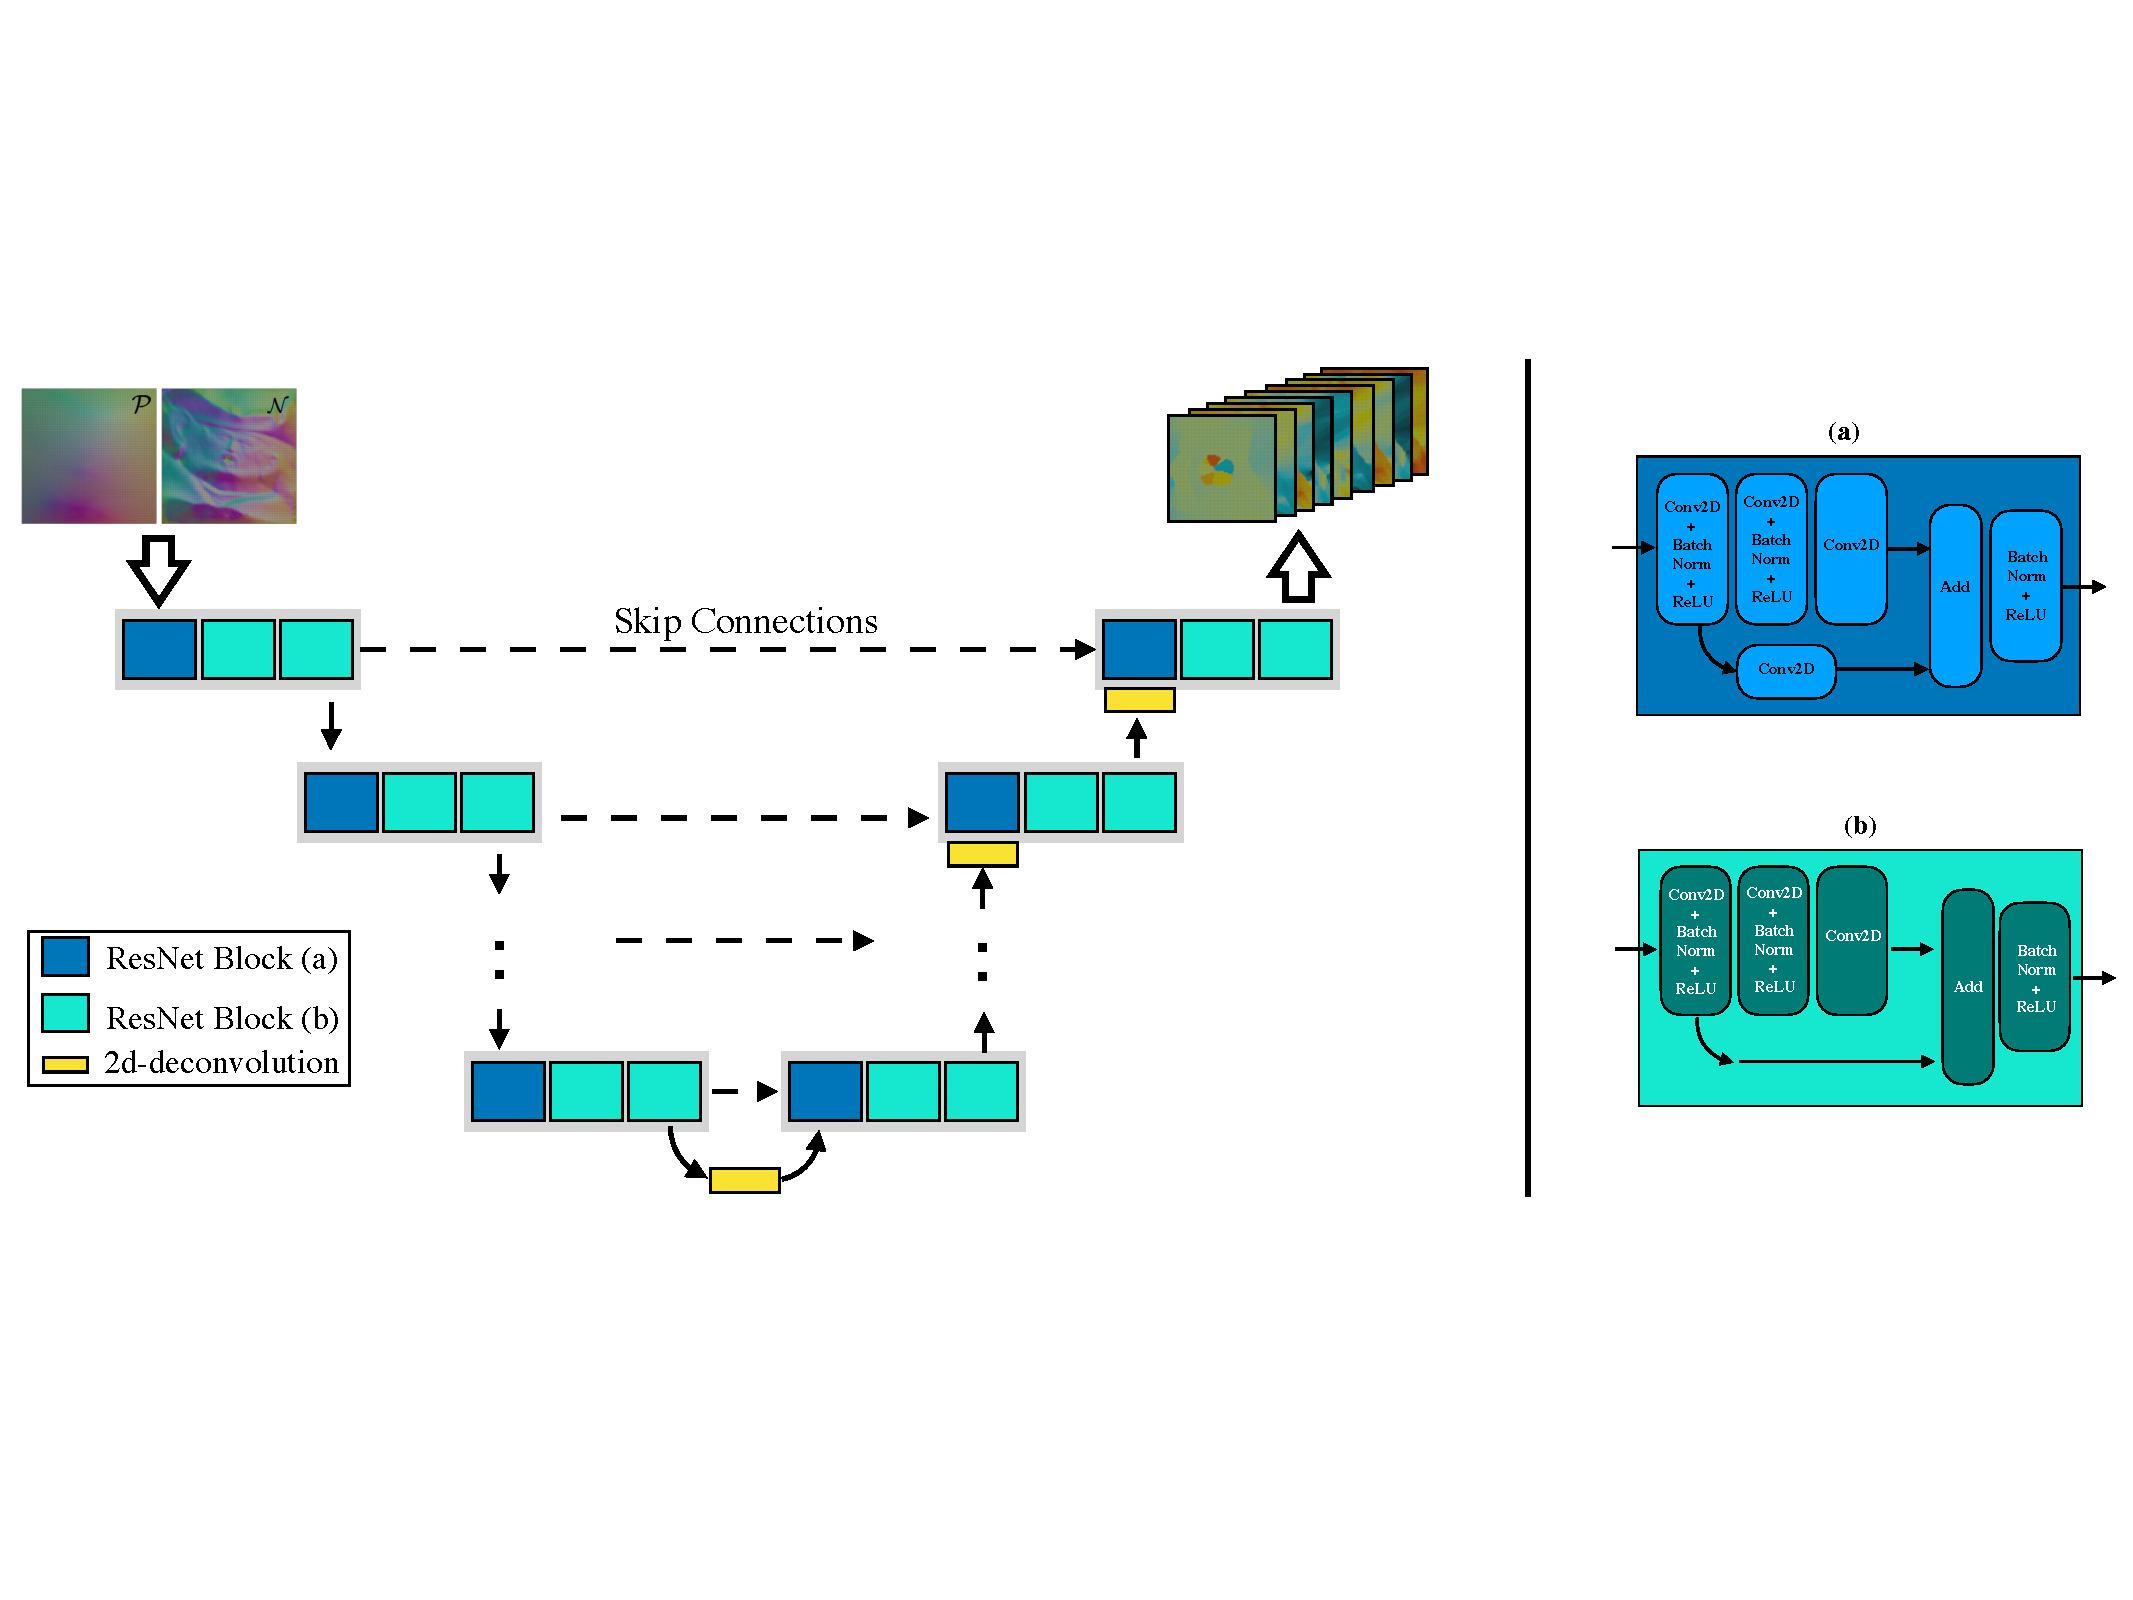
\includegraphics[width=0.7\paperwidth]{Figures/Network_topology.pdf}
     \caption{Network Topology}
     \label{Fig: NetworkTopology}
\end{figure*}

  


